\documentclass[a4,12pt]{article}
\usepackage{amsmath,amsthm,amssymb}
\usepackage{mathrsfs}
\usepackage{tikz}
\usepackage{calc}
\usepackage{comment}
%\usepackage{tikz-cd}
%\usepackage{color}
\usepackage{xcolor}
%\usepackage[usenames,dvipsnames]{xcolor}
%\usepackage[dvipdfmx]{xcolor}
\usepackage{graphicx}
%\usepackage[dvipdfmx]{graphicx}
%clash

\definecolor{NewGreen}{rgb}{0,1,0}
\definecolor{DarkGreen}{rgb}{0,0.5,0.2}
\colorlet{green}{DarkGreen}
\colorlet{lightgreen}{NewGreen}

%\usetikzlibrary{calc,intersections,through,backgrounds}
\usetikzlibrary{calc,intersections}

\usetikzlibrary{arrows.meta} % arrows={->[length=10mm]}を有効にする

\begin{document}

\begin{comment}

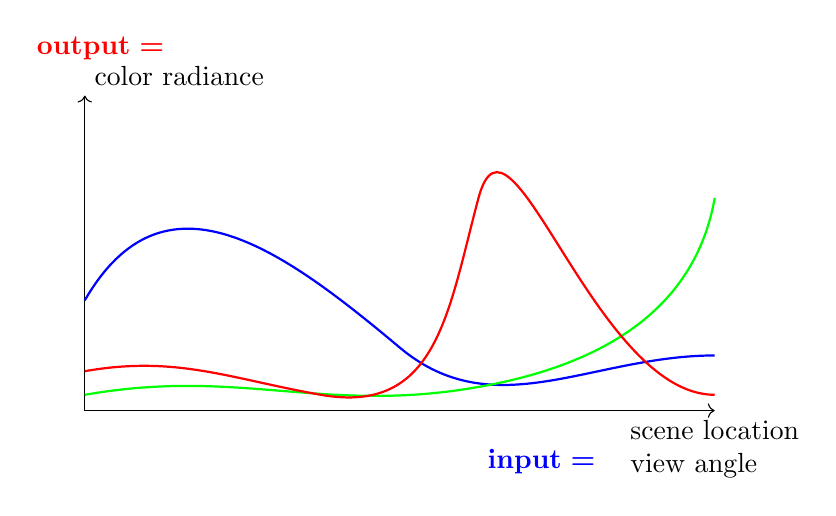
\begin{tikzpicture}

\draw[->] (0, 0) --++ (8, 0) node[below, align=left] {scene location\\view angle};
\draw[->] (0, 0) --++ (0, 4) node[above right] {color radiance};
\node at (5.8, -0.65) {\bf \color{blue} input\;=};
\node at (0.2, 4.6) {\bf \color{red} output\;=};

\draw[thick,blue,auto] (0, 1.4) to [min distance=20mm,out=60,in=140,looseness=1] (4, 0.8) to [min distance=10mm,out=-40,in=180,looseness=1] (8, 0.7);
\draw[thick,lightgreen,auto] (0, 0.2) to [min distance=20mm,out=10,in=190,looseness=1] (5, 0.3) to [min distance=10mm,out=10,in=-100,looseness=1] (8, 2.7);
\draw[thick,red,auto] (0, 0.5) to [min distance=10mm,out=10,in=170,looseness=1] (3, 0.2) to [min distance=15mm,out=-10,in=-105,looseness=1] (5, 2.7) to [min distance=10mm,out=75,in=180,looseness=1] (8, 0.2);
\end{tikzpicture}

\vspace{2mm}

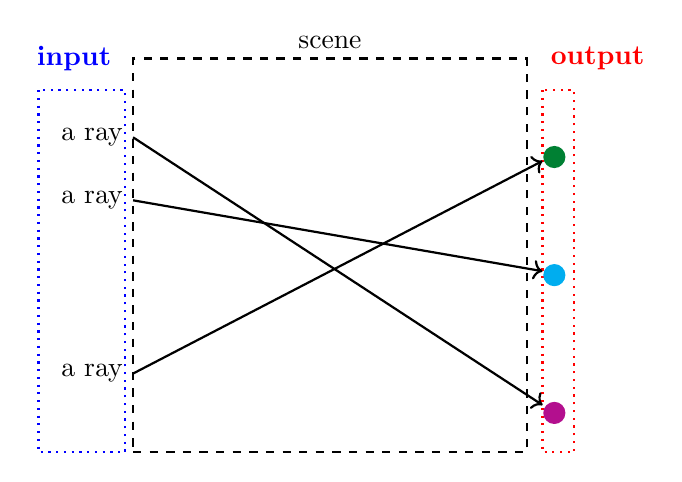
\begin{tikzpicture}
\draw[thick, dashed] (0, 0) -- (5, 0) -- (5, 5) -- (0, 5) -- cycle;
\node[above] at (2.5, 5) {scene};

\node at (-0.75, 5) {\bf \color{blue} input};
\node at (5.9, 5) {\bf \color{red} output};
\draw[blue, thick, dotted] (-1.2, 4.6) -- (-1.2, 0.0) -- (-0.1, 0.0) -- (-0.1, 4.6) -- cycle;
\draw[red, thick, dotted] (5.2, 4.6) -- (5.2, 0.0) -- (5.6, 0.0) -- (5.6, 4.6) -- cycle;

\draw[thick, ->] (0, 1.0) node[left] {a ray} -- (5.2, 3.7);
\fill[green] (5.35, 3.75) circle (4pt);

\draw[thick, ->] (0, 4.0) node[left] {a ray} -- (5.2, 0.6);
\fill[magenta!70!blue] (5.35, 0.5) circle (4pt);

\draw[thick, ->] (0, 3.2) node[left] {a ray} -- (5.2, 2.3);
\fill[cyan] (5.35, 2.25) circle (4pt);
\end{tikzpicture}




\tikzset{%
	add/.style args={#1 and #2}{
		to path={%
			($(\tikztostart)!-#1!(\tikztotarget)$)--($(\tikztotarget)!-#2!(\tikztostart)$)%
			\tikztonodes},add/.default={.2 and .2}}
}

\definecolor{ColorP}{rgb}{1.0, 0.3, 0.0}
\definecolor{ColorX}{rgb}{0.0, 1.0, 0.0}
\definecolor{ColorY}{rgb}{0.0, 0.0, 1.0}

\colorlet{ColorA}{ColorX!20!ColorY}
\colorlet{ColorB}{ColorX!40!ColorY}
\colorlet{ColorC}{ColorX!60!ColorY}
\colorlet{ColorD}{ColorX!80!ColorY}


\begin{tikzpicture}
\coordinate (P) at (3.2, 5.4);
\coordinate (S1) at (0.0, 4.5);
\coordinate (S2) at (8.0, 4.5);
\coordinate (U1) at (0.0, 3.0);
\coordinate (U2) at (8.0, 3.0);

\fill[ColorP] (P) circle (3pt) node[ColorP, above right] {point $P$};

% two planes
\draw[darkgray, thick, name path=S1--S2] (S1) node [left] {$s$ \scriptsize \rm{coordinate}} -- (S2);
\draw[darkgray, thick, name path=U1--U2] (U1) node [left] {$u$ \scriptsize \rm{coordinate}} -- (U2);

% intersections at u-plane
\coordinate (UA) at ($(U1)!0.2!(U2)$);
\coordinate (UB) at ($(U1)!0.4!(U2)$);
\coordinate (UC) at ($(U1)!0.6!(U2)$);
\coordinate (UD) at ($(U1)!0.8!(U2)$);

\fill[black] (UA) circle (1pt) node [black,below] {\scriptsize $\quad u_{A}$};
\fill[black] (UB) circle (1pt) node [black,below] {\scriptsize $\qquad u_{B}$};
\fill[black] (UC) circle (1pt) node [black,below] {\scriptsize $u_{C}\;\;$};
\fill[black] (UD) circle (1pt) node [black,below] {\scriptsize $u_{D}$};

% rays
\draw[add= .0 and .4, ColorA, thin, name path=P--UA] (P) to (UA) node [below] {$\ell_{A}$};
\draw[add= .0 and .4, ColorB, thin, name path=P--UB] (P) to (UB) node [below] {$\ell_{B}$};
\draw[add= .0 and .4, ColorC, thin, name path=P--UC] (P) to (UC) node [below] {$\ell_{C}$};
\draw[add= .0 and .4, ColorD, thin, name path=P--UD] (P) to (UD) node [below] {$\ell_{D}$};

\fill[black, name intersections={of=P--UA and S1--S2, by=SA}] (SA) circle (1pt) node [black,above] {\scriptsize $s_{A}\;\;$};
\fill[black, name intersections={of=P--UB and S1--S2, by=SB}] (SB) circle (1pt) node [black,below] {\scriptsize $s_{B}$ \quad\qquad};
\fill[black, name intersections={of=P--UC and S1--S2, by=SC}] (SC) circle (1pt) node [black,below] {\scriptsize $s_{C}\;\;$};
\fill[black, name intersections={of=P--UD and S1--S2, by=SD}] (SD) circle (1pt) node [black,above] {\scriptsize $s_{D}$};
\end{tikzpicture}

\vspace{1cm}

\begin{tikzpicture}
\coordinate (A) at (1.6, 2.6);
\coordinate (B) at (3.2, 3.2);
\coordinate (C) at (4.8, 3.8);
\coordinate (D) at (6.4, 4.4);

\coordinate (O) at (0.0, 0.0);
\coordinate (S) at (0.0, 6.0);
\coordinate (U) at (8.0, 0.0);

\draw[black, thin, name path=Saxis] (O) -- (S) node [above] {$s$};
\draw[black, thin, name path=Uaxis] (O) -- (U) node [right] {$u$};

% u軸への垂線と座標
\draw[thick, dotted] (A) -- ($(O)!(A)!(U)$) node[below] {$u_{A}$};
\draw[thick, dotted] (B) -- ($(O)!(B)!(U)$) node[below] {$u_{B}$};
\draw[thick, dotted] (C) -- ($(O)!(C)!(U)$) node[below] {$u_{C}$};
\draw[thick, dotted] (D) -- ($(O)!(D)!(U)$) node[below] {$u_{D}$};

% s軸への垂線と座標
\draw[thick, dotted] (A) -- ($(O)!(A)!(S)$) node[left] {$s_{A}$};
\draw[thick, dotted] (B) -- ($(O)!(B)!(S)$) node[left] {$s_{B}$};
\draw[thick, dotted] (C) -- ($(O)!(C)!(S)$) node[left] {$s_{C}$};
\draw[thick, dotted] (D) -- ($(O)!(D)!(S)$) node[left] {$s_{D}$};

% ray point
\fill[ColorA] (A) circle (4pt) node[ColorA, below right] {\rm ray $A$};
\fill[ColorB] (B) circle (4pt) node[ColorB, below right] {\rm ray $B$};
\fill[ColorC] (C) circle (4pt) node[ColorC, below right] {\rm ray $C$};
\fill[ColorD] (D) circle (4pt) node[ColorD, below right] {\rm ray $D$};
\end{tikzpicture}

\pagebreak




\begin{tikzpicture}
\coordinate (P) at (3.2, 5.4);
\coordinate (S1) at (0.0, 4.5);
\coordinate (S2) at (8.0, 4.5);
\coordinate (U1) at (0.0, 3.0);
\coordinate (U2) at (8.0, 3.0);

%\draw[thick, dashed, <->, magenta] (0.8, 5.4) node[above, align=center]{object\\location change} -- (7.2, 5.4);
\fill[ColorP] (P) circle (3pt) node[ColorP, above right] {point $P$};

% two planes
\draw[darkgray, thick, name path=S1--S2] (S1) node [left] {$s$ \scriptsize \rm{coordinate}} -- (S2);
\draw[darkgray, thick, name path=U1--U2] (U1) node [left] {$u$ \scriptsize \rm{coordinate}} -- (U2);

% intersections at u-plane
\coordinate (UA) at ($(U1)!0.2!(U2)$);
\coordinate (UB) at ($(U1)!0.4!(U2)$);
\coordinate (UC) at ($(U1)!0.6!(U2)$);
\coordinate (UD) at ($(U1)!0.8!(U2)$);

\fill[black] (UA) circle (1pt) node [black,below] {\scriptsize $\quad u_{A}$};
\fill[black] (UB) circle (1pt) node [black,below] {\scriptsize $\qquad u_{B}$};
\fill[black] (UC) circle (1pt) node [black,below] {\scriptsize $u_{C}\;\;$};
\fill[black] (UD) circle (1pt) node [black,below] {\scriptsize $u_{D}$};

% rays
\draw[add= .0 and .4, ColorA, thin, name path=P--UA] (P) to (UA) node [below] {$\ell_{A}$};
\draw[add= .0 and .4, ColorB, thin, name path=P--UB] (P) to (UB) node [below] {$\ell_{B}$};
\draw[add= .0 and .4, ColorC, thin, name path=P--UC] (P) to (UC) node [below] {$\ell_{C}$};
\draw[add= .0 and .4, ColorD, thin, name path=P--UD] (P) to (UD) node [below] {$\ell_{D}$};

\draw[thick, dashed, <->, ColorP] (0.0, 1.3) -- node[below]{ray angle change} (8.0, 1.3);

\fill[black, name intersections={of=P--UA and S1--S2, by=SA}] (SA) circle (1pt) node [black,above] {\scriptsize $s_{A}\;\;$};
\fill[black, name intersections={of=P--UB and S1--S2, by=SB}] (SB) circle (1pt) node [black,below] {\scriptsize $s_{B}$ \quad\qquad};
\fill[black, name intersections={of=P--UC and S1--S2, by=SC}] (SC) circle (1pt) node [black,below] {\scriptsize $s_{C}\;\;$};
\fill[black, name intersections={of=P--UD and S1--S2, by=SD}] (SD) circle (1pt) node [black,above] {\scriptsize $s_{D}$};
\end{tikzpicture}

\vspace{1cm}

\begin{tikzpicture}
\coordinate (A) at (1.6, 2.6);
\coordinate (B) at (3.2, 3.2);
\coordinate (C) at (4.8, 3.8);
\coordinate (D) at (6.4, 4.4);

\coordinate (O) at (0.0, 0.0);
\coordinate (S) at (0.0, 6.0);
\coordinate (U) at (8.0, 0.0);

\draw[black, thin, name path=Saxis] (O) -- (S) node [above] {$s$};
\draw[black, thin, name path=Uaxis] (O) -- (U) node [right] {$u$};

% u軸への垂線と座標
\draw[thick, dotted] (A) -- ($(O)!(A)!(U)$) node[below] {$u_{A}$};
\draw[thick, dotted] (B) -- ($(O)!(B)!(U)$) node[below] {$u_{B}$};
\draw[thick, dotted] (C) -- ($(O)!(C)!(U)$) node[below] {$u_{C}$};
\draw[thick, dotted] (D) -- ($(O)!(D)!(U)$) node[below] {$u_{D}$};

% s軸への垂線と座標
\draw[thick, dotted] (A) -- ($(O)!(A)!(S)$) node[left] {$s_{A}$};
\draw[thick, dotted] (B) -- ($(O)!(B)!(S)$) node[left] {$s_{B}$};
\draw[thick, dotted] (C) -- ($(O)!(C)!(S)$) node[left] {$s_{C}$};
\draw[thick, dotted] (D) -- ($(O)!(D)!(S)$) node[left] {$s_{D}$};

% 角度方向の変化
\draw[add= .3  and .3, ColorP, thick, dashed, <->, name path=view] (A) to (D) node[above left] {ray angle change};

% ray point
\fill[ColorA] (A) circle (4pt) node[ColorA, below right] {\rm ray $A$};
\fill[ColorB] (B) circle (4pt) node[ColorB, below right] {\rm ray $B$};
\fill[ColorC] (C) circle (4pt) node[ColorC, below right] {\rm ray $C$};
\fill[ColorD] (D) circle (4pt) node[ColorD, below right] {\rm ray $D$};
\end{tikzpicture}




\pagebreak
\begin{tikzpicture}
\coordinate (P) at (3.2, 5.4);
\coordinate (S1) at (0.0, 4.5);
\coordinate (S2) at (8.0, 4.5);
\coordinate (U1) at (0.0, 3.0);
\coordinate (U2) at (8.0, 3.0);

\draw[thick, dashed, <->, magenta] (0.8, 5.4) node[above, align=center]{object's\\horizontal change} -- (7.2, 5.4);
\draw[thick, dashed, <->, cyan] (3.3, 6.2) node[above, align=center]{object's\\vertical change} -- (3.3, 3.8);
\fill[ColorP] (P) circle (3pt);% node[ColorP, above right] {point $P$};

% two planes
\draw[darkgray, thick, name path=S1--S2] (S1) node [left] {$s$ \scriptsize \rm{coordinate}} -- (S2);
\draw[darkgray, thick, name path=U1--U2] (U1) node [left] {$u$ \scriptsize \rm{coordinate}} -- (U2);

% intersections at u-plane
\coordinate (UA) at ($(U1)!0.2!(U2)$);
\coordinate (UB) at ($(U1)!0.4!(U2)$);
\coordinate (UC) at ($(U1)!0.6!(U2)$);
\coordinate (UD) at ($(U1)!0.8!(U2)$);

\fill[black] (UA) circle (1pt) node [black,below] {\scriptsize $\quad u_{A}$};
\fill[black] (UB) circle (1pt) node [black,below] {\scriptsize $\qquad u_{B}$};
\fill[black] (UC) circle (1pt) node [black,below] {\scriptsize $u_{C}\;\;$};
\fill[black] (UD) circle (1pt) node [black,below] {\scriptsize $u_{D}$};

% rays
\draw[add= .0 and .4, ColorA, thin, name path=P--UA] (P) to (UA) node [below] {$\ell_{A}$};
\draw[add= .0 and .4, ColorB, thin, name path=P--UB] (P) to (UB) node [below] {$\ell_{B}$};
\draw[add= .0 and .4, ColorC, thin, name path=P--UC] (P) to (UC) node [below] {$\ell_{C}$};
\draw[add= .0 and .4, ColorD, thin, name path=P--UD] (P) to (UD) node [below] {$\ell_{D}$};

\draw[thick, dashed, <->, ColorP] (0.0, 1.3) -- node[below]{changing rays through P} (8.0, 1.3);

\fill[black, name intersections={of=P--UA and S1--S2, by=SA}] (SA) circle (1pt) node [black,above] {\scriptsize $s_{A}\;\;$};
\fill[black, name intersections={of=P--UB and S1--S2, by=SB}] (SB) circle (1pt) node [black,below] {\scriptsize $s_{B}$ \quad\qquad};
\fill[black, name intersections={of=P--UC and S1--S2, by=SC}] (SC) circle (1pt) node [black,below] {\scriptsize $s_{C}\;\;$};
\fill[black, name intersections={of=P--UD and S1--S2, by=SD}] (SD) circle (1pt) node [black,above] {\scriptsize $s_{D}$};
\end{tikzpicture}

\vspace{1cm}

\begin{tikzpicture}
\coordinate (A) at (1.6, 2.6);
\coordinate (B) at (3.2, 3.2);
\coordinate (C) at (4.8, 3.8);
\coordinate (D) at (6.4, 4.4);

\coordinate (O) at (0.0, 0.0);
\coordinate (S) at (0.0, 6.0);
\coordinate (U) at (8.0, 0.0);

\draw[black, thin, name path=Saxis] (O) -- (S) node [above] {$s$};
\draw[black, thin, name path=Uaxis] (O) -- (U) node [right] {$u$};

% u軸への垂線と座標
\draw[thick, dotted] (A) -- ($(O)!(A)!(U)$) node[below] {$u_{A}$};
\draw[thick, dotted] (B) -- ($(O)!(B)!(U)$) node[below] {$u_{B}$};
\draw[thick, dotted] (C) -- ($(O)!(C)!(U)$) node[below] {$u_{C}$};
\draw[thick, dotted] (D) -- ($(O)!(D)!(U)$) node[below] {$u_{D}$};

% s軸への垂線と座標
\draw[thick, dotted] (A) -- ($(O)!(A)!(S)$) node[left] {$s_{A}$};
\draw[thick, dotted] (B) -- ($(O)!(B)!(S)$) node[left] {$s_{B}$};
\draw[thick, dotted] (C) -- ($(O)!(C)!(S)$) node[left] {$s_{C}$};
\draw[thick, dotted] (D) -- ($(O)!(D)!(S)$) node[left] {$s_{D}$};

% 角度方向の変化
\draw[add= .3  and .3, ColorP, thick, name path=view] (A) to (D) node[above left] {rays through $P$};

\draw[magenta, thick, dashed, <->] (2.9, 1) to (2.9, 4.8) node[above] {inception change};
\draw[cyan, thick, dashed, <->] ($(3.2, 3.2)+(-5:5.5)$) arc (-5:35:5.5) node[above] {slop change};

% ray point
\fill[ColorA] (A) circle (4pt) node[ColorA, below right] {\rm ray $A$};
\fill[ColorB] (B) circle (4pt) node[ColorB, below right] {\rm ray $B$};
\fill[ColorC] (C) circle (4pt) node[ColorC, below right] {\rm ray $C$};
\fill[ColorD] (D) circle (4pt) node[ColorD, below right] {\rm ray $D$};
\end{tikzpicture}



\begin{tikzpicture}
\node (I) at (0, 0) {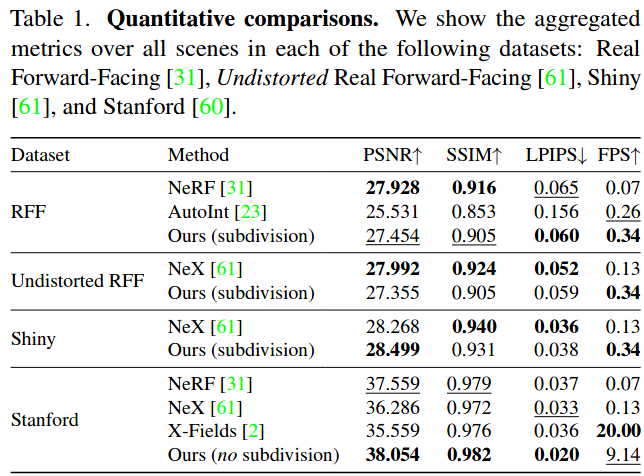
\includegraphics[width=100mm]{paper/quantitative_comparison.png}};

\def\h{5.4}
\def\wa{3.7}
\def\wb{0.8}
\def\x1{0.5}
\def\y1{1.65}
\draw[thick, blue] (\x1, \y1) --++ (0, -\h) -- node[below] {\large quality} ++ (\wa, 0) --++ (0, \h) -- cycle;
\draw[thick, orange] (\x1+\wa+0.1, \y1) --++ (0, -\h) -- node[below] {\large speed} ++ (\wb, 0) --++ (0, \h) -- cycle;

\def\h2{0.37}
\def\w3{7.7}
\def\x2{-2.5}
\draw[thick, red, dashed] (\x2,  0.2) --++ (0, -\h2) --++ (\w3, 0) --++ (0, \h2) -- cycle;
\draw[thick, red, dashed] (\x2, -0.7) --++ (0, -\h2) --++ (\w3, 0) --++ (0, \h2) -- cycle;
\draw[thick, red, dashed] (\x2, -3.2) --++ (0, -\h2) --++ (\w3, 0) --++ (0, \h2) -- cycle;
\end{tikzpicture}



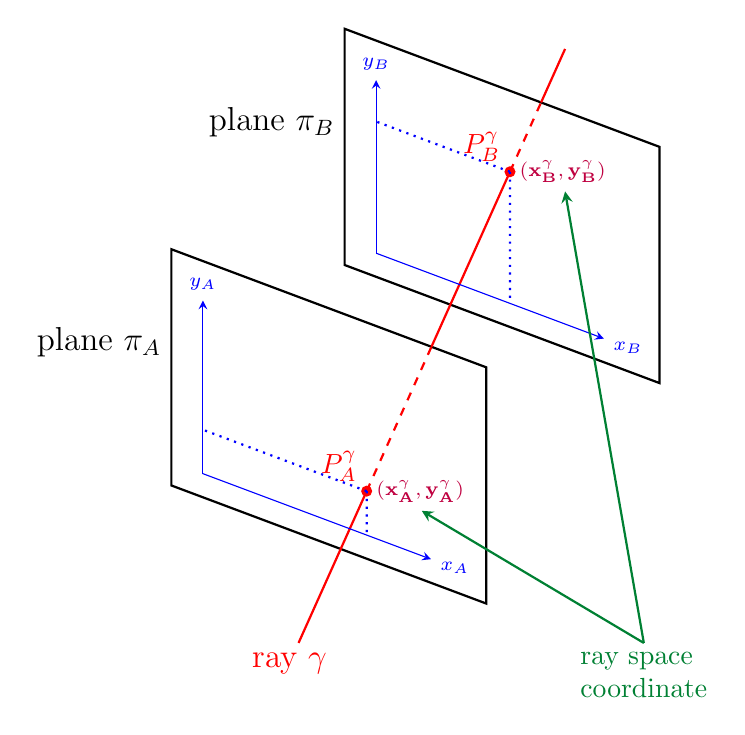
\begin{tikzpicture}
% two planes
\def\h{3}
\def\w{4}
\def\hd{1.5}
\draw[thick] (0, 0) coordinate (A1) --++ (\w, -\hd) coordinate (A2) --++ (0, \h) coordinate (A3) --++ (-\w, \hd) coordinate (A4) -- node[above left] {\large plane $\pi_A$} cycle;
\draw[thick] (2.2, 2.8) coordinate (B1) --++ (\w, -\hd) coordinate (B2) --++ (0, \h) coordinate (B3) --++ (-\w, \hd) coordinate (B4) -- node[above left] {\large plane $\pi_B$} cycle;

% line end point def
\node[red, below] (P1) at (1.5, -2) {\large ray $\gamma$};
\coordinate (P2) at ($(P1)+(3.5, 7.8)$);

% intersection
\coordinate (PA) at ($(P1)!0.28!(P2)$);
\coordinate (PB) at ($(P1)!0.8!(P2)$);
\fill[red] (PA) circle (2pt) node[above left] {$P^\gamma_A$};
\fill[red] (PB) circle (2pt) node[above left] {$P^\gamma_B$};
\node[purple, right] at (PA) {\scriptsize $\mathbf{(x_A^\gamma, y_A^\gamma)}$};
\node[purple, right] at (PB) {\scriptsize $\mathbf{(x_B^\gamma, y_B^\gamma)}$};

% line drawing
\coordinate (PAE) at (intersection of A3--A4 and P1--P2);
\coordinate (PBE) at (intersection of B3--B4 and P1--P2);
\draw[red, thick] (P1) -- (PA);
\draw[red, thick, dashed] (PA) -- (PAE);
\draw[red, thick] (PAE) -- (PB);
\draw[red, thick, dashed] (PB) -- (PBE);
\draw[red, thick] (PBE) -- (P2);

%coodinate axis
\coordinate (AO) at ($(A1)!0.1!(A3)$);
\node[blue] (AX) at ($(A2)!0.1!(A4)$) {\scriptsize $x_A$};
\node[blue] (AY) at ($(A2)!0.9!(A4)$) {\scriptsize $y_A$};
\draw[blue, thin, -stealth] (AO) -- (AX);
\draw[blue, thin, -stealth] (AO) -- (AY);

\coordinate (BO) at ($(B1)!0.1!(B3)$);
\node[blue] (BX) at ($(B2)!0.1!(B4)$) {\scriptsize $x_B$};
\node[blue] (BY) at ($(B2)!0.9!(B4)$) {\scriptsize $y_B$};
\draw[blue, thin, -stealth] (BO) -- (BX);
\draw[blue, thin, -stealth] (BO) -- (BY);

%coordinate position
\coordinate (tmpPAx) at ($(PA)+(0, -\h)$);
\coordinate (tmpPAy) at ($(PA)+(0-\w, \hd)$);
\coordinate (PAX) at (intersection of PA--tmpPAx and AO--AX);
\coordinate (PAY) at (intersection of PA--tmpPAy and AO--AY);

\draw[blue, thick, dotted] (PA) -- (PAX);% node[right, align=left] {\scriptsize $\;x_A^\gamma$};% node[above right]
\draw[blue, thick, dotted] (PA) -- (PAY);% node[above] {\scriptsize $\quad\; y_A^\gamma$};


\coordinate (tmpPBx) at ($(PB)+(0, -\h)$);
\coordinate (tmpPBy) at ($(PB)+(0-\w, \hd)$);
\coordinate (PBX) at (intersection of PB--tmpPBx and BO--BX);
\coordinate (PBY) at (intersection of PB--tmpPBy and BO--BY);

\draw[blue, thick, dotted] (PB) -- (PBX);
\draw[blue, thick, dotted] (PB) -- (PBY);

\coordinate (EXP) at (6, -2);
\draw[green, thick, -stealth] (EXP) to ($(PA) + (0.7, -0.25)$);
\draw[green, thick, -stealth] (EXP) to ($(PB) + (0.7, -0.25)$);
\node[green, below, align=left] at (EXP) {ray space\\coordinate};
\end{tikzpicture}



\pagebreak

\definecolor{wheat}{rgb}{0.93, 0.88, 0.72}
\colorlet{brightgreen}{teal!50!lightgreen}

\begin{tikzpicture}
\def\L{4}
\fill[gray] (-\L,\L) -- (-\L,-\L) -- (\L,-\L) -- (\L,\L) -- cycle;

\def\R{2.1}
\draw[magenta, thick, dotted] (-\R,\R) -- (-\R,-\R) -- (\R,-\R) -- (\R,\R) -- cycle;
\node[magenta!70!red, below] at (-2, -2.1) {\small Scene};

\node (I) at (0, 0) {\includegraphics[width=45mm]{nerf_data/lego_r_73.png}};
%\draw[blue] (1,1) -- (1,-1) -- (-1,-1) -- (-1,1) -- cycle;

\coordinate (A) at (-1, 1);
\draw[thick, yellow!95!orange, -stealth] (A) --++ (130:2.5);
\draw[thick, yellow!75!orange, -stealth] (A) --++ (150:2.5);
\draw[thick, yellow!55!orange, -stealth] (A) --++ (185:2.5);
\draw[brightgreen] (A) circle (2pt);

\coordinate (B) at (-1, -0.8);
\draw[thick, wheat, -stealth] (B) --++ (160:2.5);
\draw[thick, wheat, -stealth] (B) --++ (190:2.5);
\draw[thick, wheat!95!olive, -stealth] (B) --++ (280:2.5) node[above right, lime] {\scriptsize radiance};
\draw[brightgreen] (B) circle (2pt);

\coordinate (C) at (1, 0);
\draw[thick, black!80!darkgray, -stealth] (C) --++ (-100:2.5);
\draw[thick, black!80!darkgray, -stealth] (C) --++ (-60:2.5);
\draw[thick, black!80!darkgray, -stealth] (C) --++ (-20:2.5);
\draw[brightgreen] (C) circle (2pt);

\coordinate (D) at (0.81, 1.26);
\draw[thick, red!80!white, -stealth] (D) --++ (-20:2.5);
\draw[thick, red!80!white, -stealth] (D) --++ (20:2.5);
\draw[brightgreen] (D) circle (2pt);

\draw[blue, ultra thick, dashed, <->] ($(A)+(125:2.8)$) node[blue, right] {\scriptsize angle dependence} arc (125:190:2.8);

\node[brightgreen, above] (P) at (2, 3.2) {\scriptsize position dependence};
\draw[brightgreen, thin, dashed, shorten <= 2pt, shorten >= -2pt] (A) -- (P);
\draw[brightgreen, thin, dashed, shorten <= 2pt, shorten >= -2pt] (B) -- (P);
\draw[brightgreen, thin, dashed, shorten <= 2pt, shorten >= -2pt] (C) -- (P);
\draw[brightgreen, thin, dashed, shorten <= 2pt, shorten >= -2pt] (D) -- (P);
\end{tikzpicture}


\pagebreak


\begin{tikzpicture}
\def\l{1.8}

\node at (0,0)   {\includegraphics[width=40mm]{nerf_data/r_25.png}};

\node (I3) at (-2.2*\l, 4*\l) {\includegraphics[width=36mm]{nerf_data/r_31.png}}; %3
\node (I2) at (0,     4*\l)   {\includegraphics[width=36mm]{nerf_data/r_79.png}}; %2
\node (I1) at (2.2*\l,  4*\l) {\includegraphics[width=36mm]{nerf_data/r_17.png}}; %1

\coordinate (T1) at ($(I1) + (0, -1*\l)$);
\coordinate (T2) at ($(I2) + (0, -1*\l)$);
\coordinate (T3) at ($(I3) + (0, -1*\l)$);


\draw[dashed] ($(0,0)+(-\l,\l)$) --++ (0,-2*\l) --++ (2*\l,0) --++ (0,2*\l) -- cycle;
\draw[black,thin] ($(I1)+(-\l,\l)$) --++ (0,-2*\l) -- node[below right, align=center]{\quad view 3} ++ (2*\l,0) --++ (0,2*\l) -- cycle;
\draw[black,thin] ($(I2)+(-\l,\l)$) --++ (0,-2*\l) -- node[below right, align=center]{\; view 2} ++ (2*\l,0) --++ (0,2*\l) -- cycle;
\draw[black,thin] ($(I3)+(-\l,\l)$) --++ (0,-2*\l) -- node[below right, align=center]{view 1} ++ (2*\l,0) --++ (0,2*\l) -- cycle;
\draw[blue,thin] ($(I3)+(-1.05*\l,-1.05*\l)$) --++ (0, 2.1*\l) -- node[above, align=center]{known views\\input / training samples} ($(I1)+(1.05*\l,1.05*\l)$) --++ (0, -2.1*\l) -- cycle;


\def\th1{15}
\def\s1{2.5}
\def\fov1{30}
\coordinate (V1) at ({\s1*\l*cos(\th1)}, {\s1*\l*sin(\th1)});
\fill[blue] (V1) circle (2pt);
\draw[blue] (V1) --++ (\th1+180+\fov1:0.6*\s1*\l);
\draw[blue] (V1) --++ (\th1+180-\fov1:0.6*\s1*\l);
\coordinate (P1) at ({0.65*\s1*\l*cos(\th1)}, {0.65*\s1*\l*sin(\th1)});
\draw[blue] (P1) circle [x radius=0.065*\s1*\l, y radius=0.2*\s1*\l, rotate=\th1];
\draw[thick,blue,dashed,-stealth,auto,shorten <=7pt,shorten >=5pt] (V1) to [min distance=20mm,out=\th1,in=-60,looseness=1] (T1);

\def\th2{80}
\def\s2{2.1}
\def\fov2{40}
\coordinate (V2) at ({\s2*\l*cos(\th2)}, {\s2*\l*sin(\th2)});
\fill[blue] (V2) circle (2pt);
\draw[blue] (V2) --++ (\th2+180+\fov2:0.6*\s2*\l);
\draw[blue] (V2) --++ (\th2+180-\fov2:0.6*\s2*\l);
\coordinate (P2) at ({0.65*\s2*\l*cos(\th2)}, {0.65*\s2*\l*sin(\th2)});
\draw[blue] (P2) circle [x radius=0.03*\s2*\l, y radius=0.3*\s2*\l, rotate=\th2];
\draw[thick,blue,dashed,-stealth,auto,shorten <=7pt,shorten >=5pt] (V2) to [min distance=4mm,out=\th2,in=-90,looseness=0] (T2);

\def\th3{170}
\def\s3{2.4}
\def\fov3{35}
\coordinate (V3) at ({\s3*\l*cos(\th3)}, {\s3*\l*sin(\th3)});
\fill[blue] (V3) circle (2pt);
\draw[blue] (V3) --++ (\th3+180+\fov3:0.6*\s3*\l);
\draw[blue] (V3) --++ (\th3+180-\fov3:0.6*\s3*\l);
\coordinate (P3) at ({0.65*\s3*\l*cos(\th3)}, {0.65*\s3*\l*sin(\th3)});
\draw[blue] (P3) circle [x radius=0.035*\s3*\l, y radius=0.25*\s3*\l, rotate=\th3];

\draw[thick,blue,dashed,-stealth,auto,shorten <=7pt,shorten >=5pt] (V3) to [min distance=20mm,out=\th3,in=-120,looseness=1] (T3);




\node (I4) at (-2.5, -6.7) {\includegraphics[width=36mm]{nerf_data/r_66.png}};
\node[red] (J4) at ($(I4) + (5, 0)$) {\scalebox{5.0}{\bf ?}};%{\bf \fontsize{30}{0}\selectfont ?};
\coordinate (T4) at ($(J4) + (0, \l)$);

\def\th4{-45}
\def\s4{2.3}
\def\fov4{35}
\coordinate (V4) at ({\s4*\l*cos(\th4)}, {\s4*\l*sin(\th4)});
\fill[red] (V4) circle (2pt);
\draw[red] (V4) --++ (\th4+180+\fov4:0.6*\s4*\l);
\draw[red] (V4) --++ (\th4+180-\fov4:0.6*\s4*\l);
\coordinate (P4) at ({0.65*\s4*\l*cos(\th4)}, {0.65*\s4*\l*sin(\th4)});
\draw[red] (P4) circle [x radius=0.035*\s4*\l, y radius=0.25*\s4*\l, rotate=\th4];

\draw[thick,red,dashed,-stealth,auto,shorten <=7pt,shorten >=5pt] (V4) to [min distance=10mm,out=\th4,in=90,looseness=1] (T4);

\draw[black,thin] ($(I4)+(-\l,\l)$) --++ (0,-2*\l) --++ (2*\l,0) --++ (0,2*\l) -- cycle;
\draw[red,thin] ($(I4)+(-1.05*\l,1.05*\l)$) --++ (0,-2.1*\l) -- node[below]{ground truth} ++ (2.1*\l,0) --++ (0,2.1*\l) -- cycle;
\draw[red,thin,dashed] ($(J4)+(-\l,\l)$) --++ (0,-2*\l) -- node[below, align=center]{novel view\\output / prediction} ++ (2*\l,0) --++ (0,2*\l) -- cycle;


%\node at (0,-6)  {\includegraphics[width=40mm]{nerf_data/r_23.png}};
%\node at (-3,-6) {\includegraphics[width=40mm]{nerf_data/r_53.png}};
%\node at (3,-6)  {\includegraphics[width=40mm]{nerf_data/r_102.png}};
%\includegraphics[width=0.8\textwidth,natwidth=610,natheight=642]{figure/nerf_data/r_25.png}
%\includegraphics[width=100mm]{nerf_data/r_25.png}
%[width=.25\textwidth]
\end{tikzpicture}

\pagebreak

\end{comment}

\tikzset{%
	add/.style args={#1 and #2}{
		to path={%
			($(\tikztostart)!-#1!(\tikztotarget)$)--($(\tikztotarget)!-#2!(\tikztostart)$)%
			\tikztonodes},add/.default={.2 and .2}}
}

\definecolor{ColorP}{rgb}{1.0, 0.3, 0.0}
\definecolor{ColorQ}{rgb}{0.0, 0.3, 1.0}
\definecolor{ColorA}{rgb}{0.5, 0.8, 0.0}
\definecolor{ColorB}{rgb}{0.0, 0.8, 0.5}

\colorlet{ColorAP}{ColorA!40!ColorP}
\colorlet{ColorAQ}{ColorA!40!ColorQ}
\colorlet{ColorBP}{ColorB!40!ColorP}
\colorlet{ColorBQ}{ColorB!40!ColorQ}

\begin{comment}

\begin{tikzpicture}
\coordinate (P) at (1.5, 4.9);
\coordinate (Q) at (5.4, 6.2);
\coordinate (A) at (0.0, 0.0);
\coordinate (B) at (6.5, 1.7);
\coordinate (S1) at (0.0, 4.5);
\coordinate (S2) at (7.5, 4.5);
\coordinate (U1) at (0.0, 3.0);
\coordinate (U2) at (7.5, 3.0);

\draw[add= .3  and 0, ColorAP, thin, name path=A--P] (P) to node [above left] {$\ell_{AP}$} (A);
\draw[add= .2  and 0, ColorAQ, thin, name path=A--Q] (Q) to node [right] {$\;\ell_{AQ}$} (A);
\draw[add= .25 and 0, ColorBP, thin, name path=B--P] (P) to node [above left] {$\ell_{BP}\quad$} (B);
\draw[add= .25 and 0, ColorBQ, thin, name path=B--Q] (Q) to node [below right] {$\ell_{BQ}$} (B);

\fill[ColorP] (P) circle (3pt) node[ColorP, above right] {object $P$};
\fill[ColorQ] (Q) circle (3pt) node[ColorQ, right] {\; object $\;Q$};
\draw[ColorA] (A) circle (3pt) node[ColorA, right] {\; viewpoint $A$};
\draw[ColorA] (A) circle (1.5pt);
\draw[ColorB] (B) circle (3pt) node[ColorB, below] {viewpoint $B$};
\draw[ColorB] (B) circle (1.5pt);

\draw[gray, thick, name path=S1--S2] (S1) node [left] {$s$ \scriptsize \rm{coordinate}} -- (S2);
\draw[gray, thick, name path=U1--U2] (U1) node [left] {$u$ \scriptsize \rm{coordinate}} -- (U2);
%($(P)!-1.0!(Q)$) -- ($(P)!2.0!(Q)$);

\fill[black, name intersections={of=A--P and S1--S2, by=SAP}] (SAP) circle (1pt) node [black,above left] {\scriptsize $s_{AP}$};
\fill[black, name intersections={of=A--Q and S1--S2, by=SAQ}] (SAQ) circle (1pt) node [black,above] {\scriptsize $s_{AQ}\quad$};
\fill[black, name intersections={of=B--P and S1--S2, by=SBP}] (SBP) circle (1pt) node [black,above] {\scriptsize $\;s_{BP}$};
\fill[black, name intersections={of=B--Q and S1--S2, by=SBQ}] (SBQ) circle (1pt) node [black,above right] {\scriptsize $s_{BQ}$};

\fill[black, name intersections={of=A--P and U1--U2, by=UAP}] (UAP) circle (1pt) node [black,below right] {\scriptsize $u_{AP}$};
\fill[black, name intersections={of=A--Q and U1--U2, by=UAQ}] (UAQ) circle (1pt) node [black,below right] {\scriptsize $u_{AQ}$};
\fill[black, name intersections={of=B--P and U1--U2, by=UBP}] (UBP) circle (1pt) node [black,below] {\scriptsize $u_{BP}\quad$};
\fill[black, name intersections={of=B--Q and U1--U2, by=UBQ}] (UBQ) circle (1pt) node [black,below left] {\scriptsize $u_{BQ}$};
\end{tikzpicture}

\vspace{1cm}

\begin{tikzpicture}
\coordinate (AP) at (0.92, 1.38);
\coordinate (AQ) at (2.61, 3.92);
\coordinate (BP) at (4.47, 2.13);
\coordinate (BQ) at (6.18, 5.82);

\coordinate (O) at (0.0, 0.0);
\coordinate (S) at (0.0, 7.0);
\coordinate (U) at (7.0, 0.0);

\draw[black, thin, name path=Saxis] (O) -- (S) node [above] {$s$};
\draw[black, thin, name path=Uaxis] (O) -- (U) node [right] {$u$};

% u軸への垂線と座標
\draw[thick, dotted] (AP) -- ($(O)!(AP)!(U)$) node[below] {$u_{AP}$};
\draw[thick, dotted] (AQ) -- ($(O)!(AQ)!(U)$) node[below] {$u_{AQ}$};
\draw[thick, dotted] (BP) -- ($(O)!(BP)!(U)$) node[below] {$u_{BP}$};
\draw[thick, dotted] (BQ) -- ($(O)!(BQ)!(U)$) node[below] {$u_{BQ}$};

% s軸への垂線と座標
\draw[thick, dotted] (AP) -- ($(O)!(AP)!(S)$) node[left] {$s_{AP}$};
\draw[thick, dotted] (AQ) -- ($(O)!(AQ)!(S)$) node[left] {$s_{AQ}$};
\draw[thick, dotted] (BP) -- ($(O)!(BP)!(S)$) node[left] {$s_{BP}$};
\draw[thick, dotted] (BQ) -- ($(O)!(BQ)!(S)$) node[left] {$s_{BQ}$};

% ray point
\fill[ColorAP] (AP) circle (4pt) node[ColorAP, below right] {\rm ray $AP$};
\fill[ColorAQ] (AQ) circle (4pt) node[ColorAQ, above left] {\rm ray $AQ$};
\fill[ColorBP] (BP) circle (4pt) node[ColorBP, below right] {\rm ray $BP$};
\fill[ColorBQ] (BQ) circle (4pt) node[ColorBQ, above left] {\rm ray $BQ$};

%\node[shape=star, star points=5, star point ratio=1.5]

% view line
\draw[add= .3  and .3, ColorA, thick, dashed, name path=A] (AP) to (AQ) node[above] {\rm view $A$};
\draw[add= .3  and .3, ColorB, thick, dashed, name path=B] (BP) to (BQ) node[above] {\rm view $B$};
\end{tikzpicture}


\end{comment}

\vspace{1cm}

% 既存サンプルが与えられた時
\begin{tikzpicture}
\coordinate (AP) at (0.92, 1.38);
\coordinate (AQ) at (2.61, 3.92);
\coordinate (BP) at (4.47, 2.13);
\coordinate (BQ) at (6.18, 5.82);

\coordinate (O) at (0.0, 0.0);
\coordinate (S) at (0.0, 7.0);
\coordinate (U) at (7.0, 0.0);

\draw[black, thin, name path=Saxis] (O) -- (S) node [above] {$s$};
\draw[black, thin, name path=Uaxis] (O) -- (U) node [right] {$u$};

\draw[add= .3  and .3, ColorA, thick, dashed, name path=A] (AP) to (AQ) node[above] {\rm view $A$};
\draw[add= .3  and .3, ColorB, thick, dashed, name path=B] (BP) to (BQ) node[above] {\rm view $B$};

\def\p{0.12}
\fill[ColorP] ($(AP)+(-\p, -\p)$) rectangle ($(AP)+(\p, \p)$) node[ColorAP, above left] {$AP$};
\fill[ColorQ] ($(AQ)+(-\p, -\p)$) rectangle ($(AQ)+(\p, \p)$) node[ColorAQ, above left] {$AQ$};
\fill[ColorP] ($(BP)+(-\p, -\p)$) rectangle ($(BP)+(\p, \p)$) node[ColorBP, above left] {$BP$};
\fill[ColorQ] ($(BQ)+(-\p, -\p)$) rectangle ($(BQ)+(\p, \p)$) node[ColorBQ, above left] {$BQ$};
%\fill[ColorP] (AP) circle (4pt) node[ColorAP, above left] {$AP$};
%\fill[ColorQ] (AQ) circle (4pt) node[ColorAQ, above left] {$AQ$};
%\fill[ColorP] (BP) circle (4pt) node[ColorBP, above left] {$BP$};
%\fill[ColorQ] (BQ) circle (4pt) node[ColorBQ, above left] {$BQ$};
\end{tikzpicture}

\vspace{1mm}

% 未知サンプルの輝度推定
\begin{tikzpicture}
\coordinate (AP) at (0.92, 1.38);
\coordinate (AQ) at (2.61, 3.92);
\coordinate (BP) at (4.47, 2.13);
\coordinate (BQ) at (6.18, 5.82);

\coordinate (O) at (0.0, 0.0);
\coordinate (S) at (0.0, 7.0);
\coordinate (U) at (7.0, 0.0);

\draw[black, thin, name path=Saxis] (O) -- (S) node [above] {$s$};
\draw[black, thin, name path=Uaxis] (O) -- (U) node [right] {$u$};

\draw[add= .3  and .3, ColorA, thick, dashed, name path=A] (AP) to (AQ) node[above] {\rm view $A$};
\draw[add= .3  and .3, ColorB, thick, dashed, name path=B] (BP) to (BQ) node[above] {\rm view $B$};

\def\p{0.12}
\fill[ColorP] ($(AP)+(-\p, -\p)$) rectangle ($(AP)+(\p, \p)$) node[ColorAP, above left] {$AP$};
\fill[ColorQ] ($(AQ)+(-\p, -\p)$) rectangle ($(AQ)+(\p, \p)$) node[ColorAQ, above left] {$AQ$};
\fill[ColorP] ($(BP)+(-\p, -\p)$) rectangle ($(BP)+(\p, \p)$) node[ColorBP, above left] {$BP$};
\fill[ColorQ] ($(BQ)+(-\p, -\p)$) rectangle ($(BQ)+(\p, \p)$) node[ColorBQ, above left] {$BQ$};

\coordinate (X) at ($(AP)!0.52!(BP)$);
\coordinate (Y) at ($(AQ)!0.42!(BQ)$);
\draw[add= .35  and .35, ultra thick, lightgray] (X) to (Y) node[above, align=center, magenta] {\bf novel\\\bf view};
\node[magenta, right] at ($(X)!-0.2!(Y)$) {\bf ?};
\node[magenta, right] at ($(X)!0.0!(Y)$)  {\bf ?};
\node[magenta, right] at ($(X)!0.2!(Y)$)  {\bf ?};
\node[magenta, right] at ($(X)!0.4!(Y)$)  {\bf ?};
\node[magenta, right] at ($(X)!0.6!(Y)$)  {\bf ?};
\node[magenta, right] at ($(X)!0.8!(Y)$)  {\bf ?};
\node[magenta, right] at ($(X)!1.0!(Y)$)  {\bf ?};
\node[magenta, right] at ($(X)!1.2!(Y)$)  {\bf ?};
\end{tikzpicture}

\vspace{1cm}

% 正解
\begin{tikzpicture}
\coordinate (AP) at (0.92, 1.38);
\coordinate (AQ) at (2.61, 3.92);
\coordinate (BP) at (4.47, 2.13);
\coordinate (BQ) at (6.18, 5.82);

\coordinate (O) at (0.0, 0.0);
\coordinate (S) at (0.0, 7.0);
\coordinate (U) at (7.0, 0.0);

\draw[black, thin, name path=Saxis] (O) -- (S) node [above] {$s$};
\draw[black, thin, name path=Uaxis] (O) -- (U) node [right] {$u$};

\draw[add= .3  and .3, ColorP, ultra thick, name path=P] (AP) to (BP) node[above right] {\rm radiance $P$};
\draw[add= .3  and .3, ColorQ, ultra thick, name path=Q] (AQ) to (BQ) node[above right] {\rm radiance $Q$};

\def\p{0.12}
\fill[ColorP] ($(AP)+(-\p, -\p)$) rectangle ($(AP)+(\p, \p)$) node[ColorAP, above left] {$AP$};
\fill[ColorQ] ($(AQ)+(-\p, -\p)$) rectangle ($(AQ)+(\p, \p)$) node[ColorAQ, above left] {$AQ$};
\fill[ColorP] ($(BP)+(-\p, -\p)$) rectangle ($(BP)+(\p, \p)$) node[ColorBP, above left] {$BP$};
\fill[ColorQ] ($(BQ)+(-\p, -\p)$) rectangle ($(BQ)+(\p, \p)$) node[ColorBQ, above left] {$BQ$};
%\fill[ColorP] (AP) circle (4pt) node[ColorAP, above left] {$AP$};
%\fill[ColorQ] (AQ) circle (4pt) node[ColorAQ, above left] {$AQ$};
%\fill[ColorP] (BP) circle (4pt) node[ColorBP, above left] {$BP$};
%\fill[ColorQ] (BQ) circle (4pt) node[ColorBQ, above left] {$BQ$};
\end{tikzpicture}

%%%

\pagebreak

\begin{tikzpicture}
\def\f{0.75}
\coordinate (CameraCenter) at (10.0, 0.0);
\coordinate (SceneCenter) at (0.0, 0.0);
\coordinate (SceneSphere) at ($(SceneCenter)+(-0.6, -0.5)$);
\coordinate (SceneCube) at ($(SceneCenter)+(1.0, 0.3)$);
\coordinate (ImagePlaneCenter) at ($(SceneCenter)!\f!(CameraCenter)$);
\coordinate (ImageSphere) at ($(SceneSphere)!\f!(CameraCenter)$);
\coordinate (ImageCube) at ($(SceneCube)!\f!(CameraCenter)$);

% Scene
\draw[blue] (SceneSphere) circle (14pt);
\def\r{0.9}
\coordinate (Cube0) at ($(SceneCube)$);
\coordinate (Cube1) at ($(SceneCube)+(0.0, 0.0)+(0, \r)$);
\coordinate (Cube2) at ($(SceneCube)+(0.0, 0.0)+(-0.866*\r, 0.5*\r)$);
\coordinate (Cube3) at ($(SceneCube)+(0.0, 0.0)+(-0.866*\r, -0.5*\r)$);
\coordinate (Cube4) at ($(SceneCube)+(0.0, 0.0)+(0, -\r)$);
\coordinate (Cube5) at ($(SceneCube)+(0.0, 0.0)+(0.866*\r, -0.5*\r)$);
\coordinate (Cube6) at ($(SceneCube)+(0.0, 0.0)+(0.866*\r, 0.5*\r)$);
\draw[blue] (Cube1) -- (Cube2) -- (Cube3) -- (Cube4) -- (Cube5) -- (Cube6) -- cycle;
\draw[blue] (Cube0) -- (Cube2);
\draw[blue] (Cube0) -- (Cube4);
\draw[blue] (Cube0) -- (Cube6);
\node[blue] at ($(SceneCenter)+(-1,1)$) {$s \in \mathscr{S}$};

% Camera
\fill[orange] (CameraCenter) circle (2pt);
\def\xc{-1.3};
\def\yc{0.65};
\def\xd{1.3};
\def\yd{1.05};
\coordinate (Plane1) at ($(ImagePlaneCenter)+(\xc,\yc)$);
\coordinate (Plane2) at ($(ImagePlaneCenter)+(\xd,\yd)$);
\coordinate (Plane3) at ($(ImagePlaneCenter)+(-\xc,-\yc)$);
\coordinate (Plane4) at ($(ImagePlaneCenter)+(-\xd,-\yd)$);
\draw[orange] (Plane1) -- (Plane2) -- (Plane3) -- (Plane4) -- cycle;
\node[orange, above right] at ($(CameraCenter)+(0,0)$) {$p \in \mathscr{P}$};
\draw[add= .0  and 2., orange, dashed] (CameraCenter) to (Plane1);
\draw[add= .0  and 1.3, orange, dashed] (CameraCenter) to (Plane2);
\draw[add= .0  and 1.5, orange, dashed] (CameraCenter) to (Plane3);
\draw[add= .0  and 1.2, orange, dashed] (CameraCenter) to (Plane4);

% 2D Image
\draw[green] (ImageSphere) circle (5.6pt);
\def\ir{0.36}
\coordinate (ICube0) at ($(ImageCube)$);
\coordinate (ICube1) at ($(ImageCube)+(0.0, -0.04*\ir)+(0, \ir)$);
\coordinate (ICube2) at ($(ImageCube)+(0.2*\ir, 0.02*\ir)+(-0.866*\ir, 0.5*\ir)$);
\coordinate (ICube3) at ($(ImageCube)+(0.3*\ir, 0.02*\ir)+(-0.866*\ir, -0.5*\ir)$);
\coordinate (ICube4) at ($(ImageCube)+(0.1*\ir, -0.02*\ir)+(0, -\ir)$);
\coordinate (ICube5) at ($(ImageCube)+(0.05*\ir, -0.03*\ir)+(0.866*\ir, -0.5*\ir)$);
\coordinate (ICube6) at ($(ImageCube)+(0.05*\ir, -0.03*\ir)+(0.866*\ir, 0.5*\ir)$);
\draw[green] (ICube1) -- (ICube2) -- (ICube3) -- (ICube4) -- (ICube5) -- (ICube6) -- cycle;
\draw[green] (ICube0) -- (ICube2);
\draw[green] (ICube0) -- (ICube4);
\draw[green] (ICube0) -- (ICube6);
\node[green, below] at ($(ImagePlaneCenter)+(0,1)$) {$o \in \mathscr{O}$};

% rendering
\coordinate (Render1) at ($(SceneCenter)!0.3!(ImagePlaneCenter)$);
\coordinate (Render2) at ($(SceneCenter)!0.75!(ImagePlaneCenter)$);
\draw[red, ultra thick, -stealth] ($(Render1)+(0,0)$) -- node[red, above, inner sep=3mm] {$\Pi$} ($(Render2)+(0,0)$);
\end{tikzpicture}


\end{document}